\documentclass[UTF8]{ctexart}

\usepackage{float}
\usepackage{graphics,graphicx,pdfpages}
\usepackage{color}
\usepackage{xcolor}
\usepackage{shapepar}
\usepackage{lettrine}
\usepackage{picinpar}


\title{\zihao{1}{\CJKfamily{kai}多功能计算器V1.0\\说\\明\\书}}
\author{\\\\\\\\\\\\{\CJKfamily{kai}美猴王}}
\date{{\CJKfamily{kai}2016年1月14日}}

\bibliographystyle{plain}

\begin{document}
\maketitle\thispagestyle{empty}

\newpage
\tableofcontents\thispagestyle{empty}

\newpage
%%%%%%%%%%%%%%%%%%%%%%%%%%%%%%%%%%%%%%%%%%%%%%%%%%%%%%%%%%%%%%%%%%%%%%%%%%
\section{开发环境与安装说明}
\subsection{开发与测试环境说明}
本软件基于Matlab R2015a平台开发并编译,于Windows10环境下测试成功。

\subsection{安装说明}
打开MultifunctionalCalculatorAppInstallermcr.exe进行安装。按照提示进行即可。
\footnote{对于初次安装的用户需要注意,安装过程会有两次路径选择提示,第一次为选择软件安装路径,第二次为选择运行环境安装路径。}
\footnote{对于已安装过该版本MATLABCompilerRuntime的计算机,会自动可跳过MCR安装步骤。}

安装过程截图如下:
\begin{figure}[H]
\centering
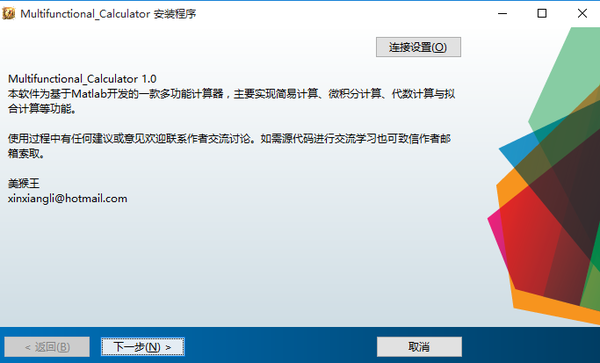
\includegraphics[scale=0.5]{image/pic001.png}
\caption{安装过程1}
\label{fig:pic001}
\end{figure}

\begin{figure}[H]
\centering
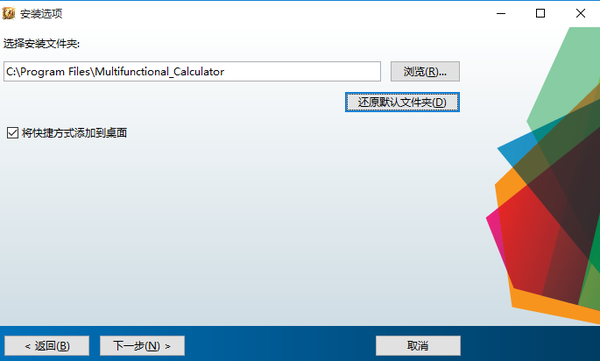
\includegraphics[scale=0.5]{image/pic002.png}
\caption{安装过程2}
\label{fig:pic002}
\end{figure}

\begin{figure}[H]
\centering
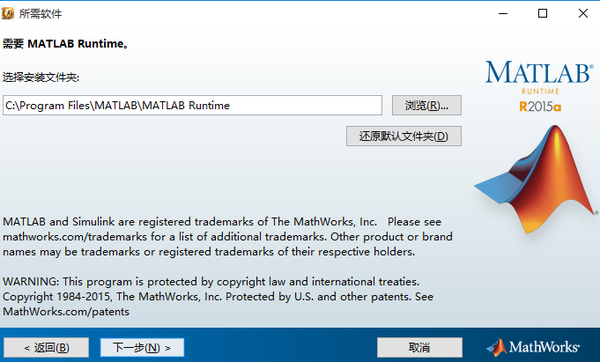
\includegraphics[scale=0.5]{image/pic003.png}
\caption{安装过程3}
\label{fig:pic003}
\end{figure}

\begin{figure}[H]
\centering
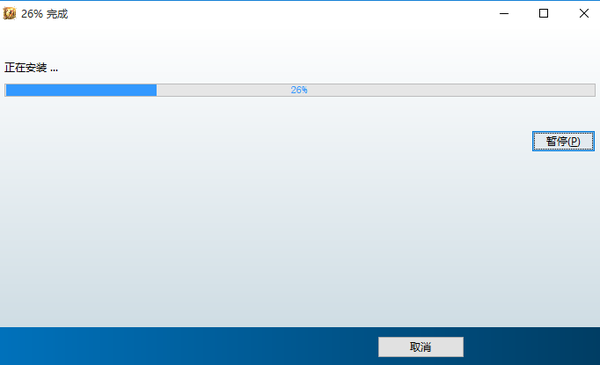
\includegraphics[scale=0.5]{image/pic004.png}
\caption{安装过程4}
\label{fig:pic004}
\end{figure}

\begin{figure}[H]
\centering
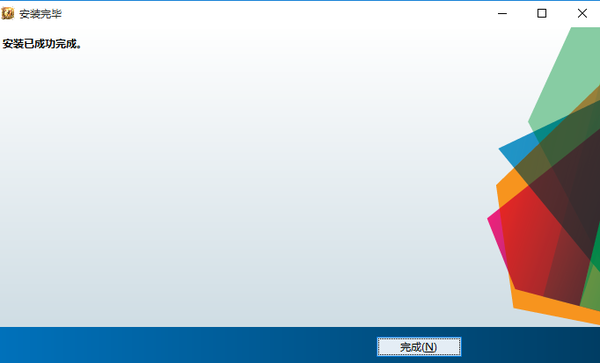
\includegraphics[scale=0.5]{image/pic005.png}
\caption{安装过程5}
\label{fig:pic005}
\end{figure}

安装完毕之后,运行桌面上的快捷方式即可。

\begin{figure}[H]
\centering
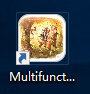
\includegraphics[scale=0.45]{image/pic006.png}
\caption{快捷方式}
\label{fig:pic006}
\end{figure}

如果在安装过程中忘记勾选添加到桌面快捷方式,只需在安装路径
(……/MultifunctionalCalculator/application)下找到MultifunctionalCalculator.exe即可。

\begin{figure}[H]
\centering
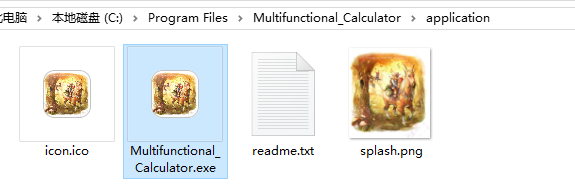
\includegraphics[scale=0.7]{image/pic007.png}
\caption{安装路径}
\label{fig:pic007}
\end{figure}


%%%%%%%%%%%%%%%%%%%%%%%%%%%%%%%%%%%%%%%%%%%%%%%%%%%%%%%%%%%%%%%%%%%%%%%%%%%%
\section{界面与功能说明}
本软件的主要有简易计算、微积分计算
\footnote{由于syms函数编译后无法调用,编译后软件已丢失微积分计算功能,如需使用请用源代码运行。}
、代数计算、拟合等功能。

\subsection{主界面}
打开软件,将弹出作者说明页。如下图所示:

\bigskip

\begin{figure}[H]
\centering
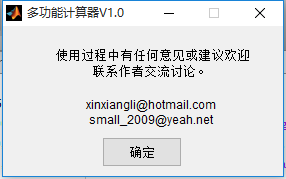
\includegraphics[scale=0.7]{image/pic01.png}
\caption{作者说明页}
\label{fig:pic01}
\end{figure}

\clearpage
单击确定后弹出主界面,如下图所示:

\bigskip

\begin{figure}[H]
\centering
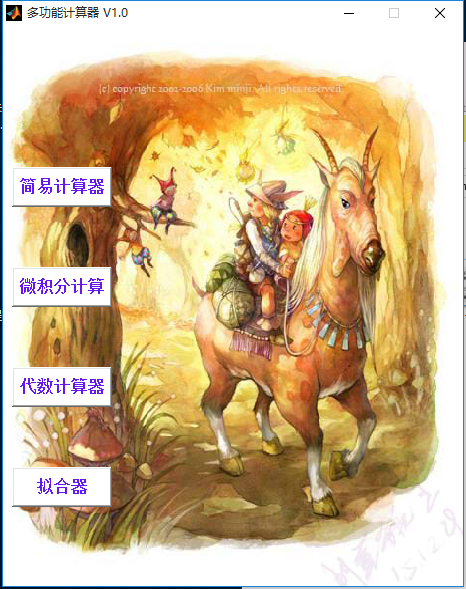
\includegraphics[scale=0.6]{image/pic02.png}
\caption{主界面}
\label{fig:pic02}
\end{figure}

\bigskip

\subsection{简易计算器}
单击简易计算器按钮弹出简易计算器功能界面,如下图所示:
\begin{figure}[H]
\centering
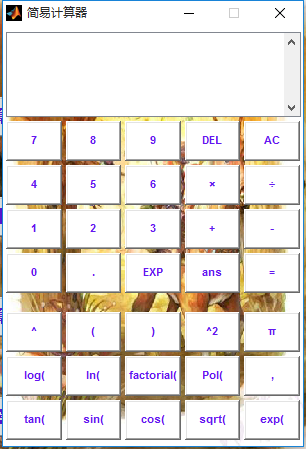
\includegraphics[scale=0.5]{image/pic03.png}
\caption{简易计算器界面}
\label{fig:pic03}
\end{figure}

\subsection{微积分计算器}
单击微积分计算器,会有微/积分计算选择对话框弹出,用户按照需求选择即可。
\footnote{该对话框不会自动关闭,以便用户同时进行微分积分计算。(微积分计算可同时打开)}

\begin{figure}[H]
\centering
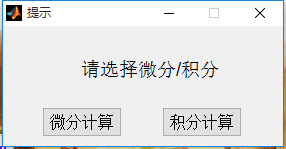
\includegraphics[scale=0.5]{image/pic04.png}
\caption{微积分计算选择对话框}
\label{fig:pic04}
\end{figure}

以微分计算为例,单击微分计算可得到微分计算界面:
\begin{figure}[H]
\centering
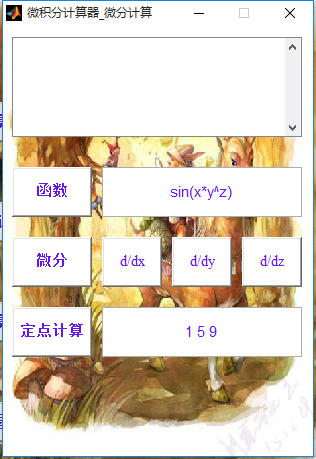
\includegraphics[scale=0.45]{image/pic05.png}
\caption{微分计算界面}
\label{fig:pic05}
\end{figure}

\subsection{代数计算器与拟合器}
代数计算器界面:
\begin{figure}[H]
\centering
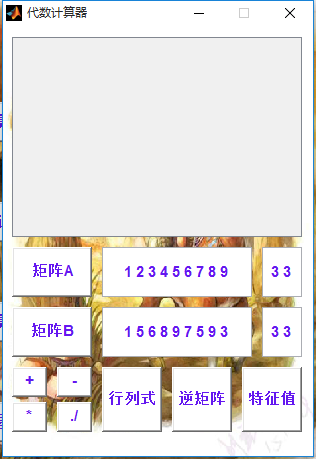
\includegraphics[scale=0.45]{image/pic06.png}
\caption{代数计算界面}
\label{fig:pic06}
\end{figure}
%%%%%%%%%%%%%%%%%%%%%%%%%%%%%%%%%%%%%%%%%%%%%%%%%%%%%%%%%%%%%%%%%%%%%%%%%%%%%%%%%%
\section{算例演示}
为方便测试与检验,程序内部已经设置默认值。现以程序缺省算例为例,介绍软件具体使用方法及注意事项。
\subsection{微积分计算器的使用}
以微分计算器为例,在呼出微分计算器界面后。在函数后的文本框内以Matlab格式输入待微分函数,
单击“函数”按钮即可于显示框内得到所输函数。
\begin{figure}[H]
\centering
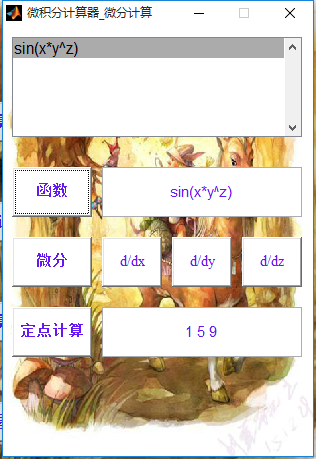
\includegraphics[scale=0.4]{image/pic08.png}
\caption{微分计算范例}
\label{fig:pic08}
\end{figure}
确认无误后即可对其进行微分计算。
\footnote{对哪个变量求微分即单击微分按钮后的$d/d$?按钮,需要求几次即单击几次。
例:如需要对函数$z=f(x,y)$求$ \partial z^3 /\partial^2 x \partial y$ 
只需输入原函数并两次点击$d/dx$一次点击$d/dy$即可得到。如图15所示。}
\begin{figure}[H]
\centering
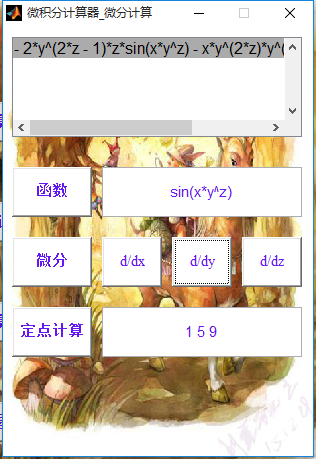
\includegraphics[scale=0.4]{image/pic09.png}
\caption{微分计算范例(计算$ \partial z^3 /\partial^2 x \partial y$)}
\label{fig:pic09}
\end{figure}
积分计算同上。

\subsection{代数计算器的使用}
首先,在矩阵A(B)按钮后面的文本框输入矩阵的元素及形状,单击矩阵A(B)进行保存,即可在显示屏幕上的得到指定形状的输入矩阵。如图16所示。
\begin{figure}[H]
\centering
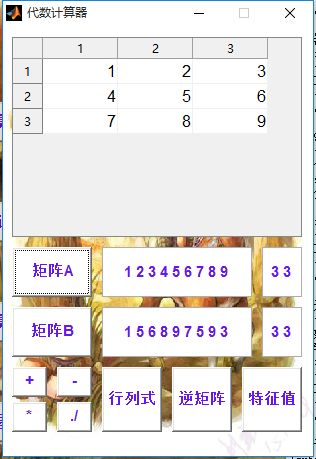
\includegraphics[scale=0.4]{image/pic10.png}
\caption{代数计算范例(矩阵输入与保存)}
\label{fig:pic10}
\end{figure}
单击左下方的四则运算符即可进行输入矩阵A、B的四则运算。
\footnote{./号表示矩阵的点除。}
如图17所示:
\footnote{图17所示即为输入矩阵A、B的加法结果。}
\begin{figure}[H]
\centering
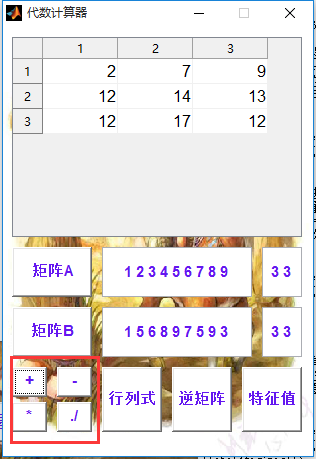
\includegraphics[scale=0.4]{image/pic11.png}
\caption{代数计算范例(输入矩阵的四则运算)}
\label{fig:pic11}
\end{figure}
其后的行列式/逆矩阵/特征值的计算为对显示屏幕的矩阵进行计算。
\footnote{注意与四则运算对象的区别。}
若矩阵不为方阵,会有如图18所示的提醒:
\begin{figure}[H]
\centering
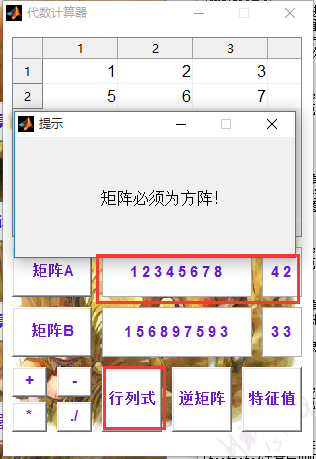
\includegraphics[scale=0.4]{image/pic12.png}
\caption{非方阵提醒}
\label{fig:pic12}
\end{figure}
若矩阵不可逆,则所求逆矩阵不可得,如图19所示:
\begin{figure}[H]
\centering
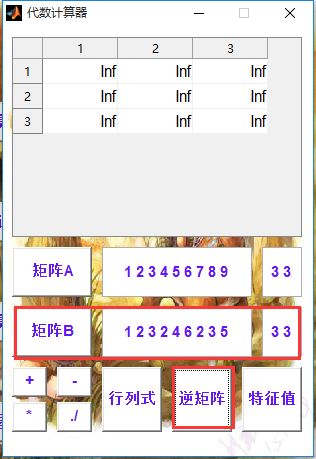
\includegraphics[scale=0.4]{image/pic13.png}
\caption{不可逆提醒}
\label{fig:pic13}
\end{figure}

\subsection{拟合器的使用}
首先用户需要依照样本格式给出拟合数据,如图20所示:
\begin{figure}[H]
\centering
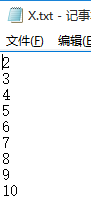
\includegraphics[scale=0.4]{image/pic14.png}
\caption{范例样本格式}
\label{fig:pic14}
\end{figure}
然后单击导入数据分别将x,y的数据导入储存,导入后即显示在显示屏矩阵输出分屏上。如图21所示:
\begin{figure}[H]
\centering
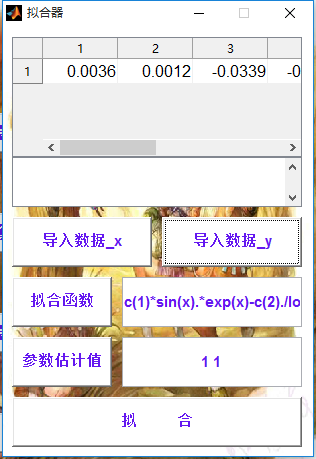
\includegraphics[scale=0.4]{image/pic15.png}
\caption{数据导入}
\label{fig:pic15}
\end{figure}
然后在“拟合函数”后的文本框内按照$Matlab$格式
\footnote{目前暂时采用用户遵守机器语言格式的形式输入,有待改进。}
输入待拟合函数,如图22所示:
\begin{figure}[H]
\centering
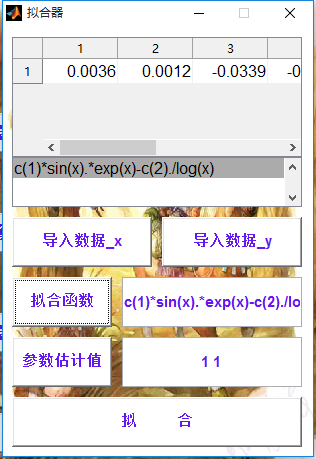
\includegraphics[scale=0.4]{image/pic16.png}
\caption{数据导入}
\label{fig:pic16}
\end{figure}
输入参数的估计值并储存。
\footnote{单击“参数估计值”按钮即可,当文本显示分屏将估计值输出即表明参数估计值已经导入。}
导入参数估计值后即单击“拟合”按钮。即可得到参数拟合结果,如图23所示
\footnote{按顺序输出参数值,即从左往右数,第一个为参数$c(1)$的拟合结果,第二个为参数$c(2)$的拟合结果}:
\begin{figure}[H]
\centering
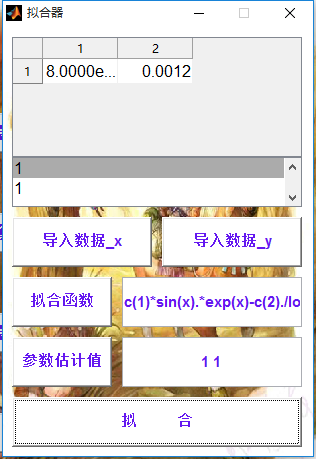
\includegraphics[scale=0.4]{image/pic17.png}
\caption{拟合结果}
\label{fig:pic17}
\end{figure}

%%%%%%%%%%%%%%%%%%%%%%%%%%%%%%%%%%%%%%%%%%%%%%%%%%%%%%%%%%
\section{结语}
感谢大家的使用并且真诚地希望各位提出宝贵的意见。
如果您在使用过程中有任何建议或意见,或者对于源代码及算法有任何疑惑,欢迎联系作者交流讨论。

作者邮箱:xinxiangli@hotmail.com
\end{document}


